\section{Strömungslinien}
	\begin{figure}
	\centering
	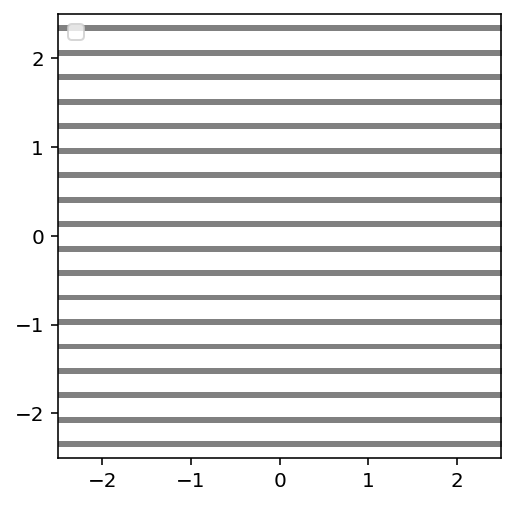
\includegraphics[width=0.45\textwidth]{papers/joukowski/images/05_stroemungslinien/Strom_g.png}
	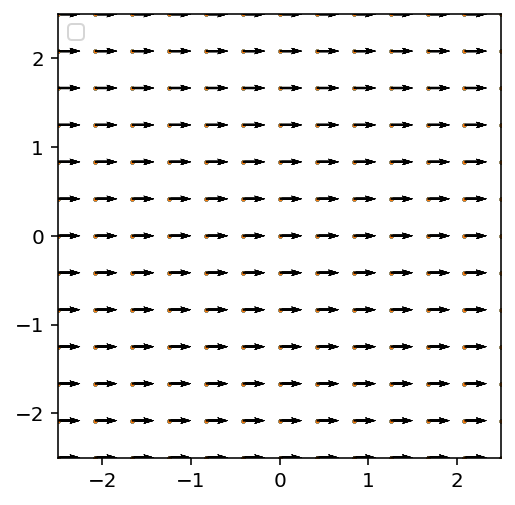
\includegraphics[width = 0.45\textwidth]{papers/joukowski/images/05_stroemungslinien/speed.png}
\end{figure}

	\begin{figure}
	\centering
	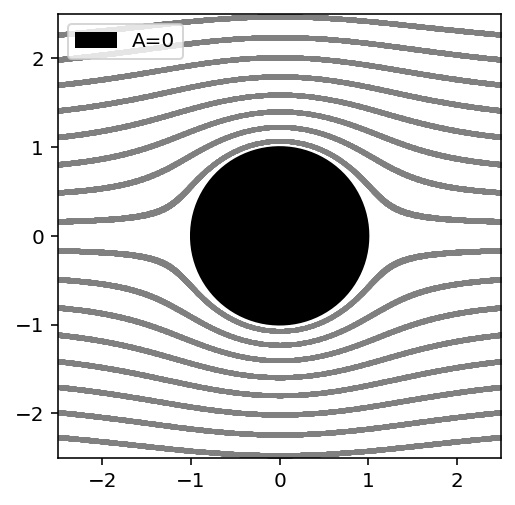
\includegraphics[width=0.45\textwidth]{papers/joukowski/images/05_stroemungslinien/Magnus_Strom_A000_g.png}
	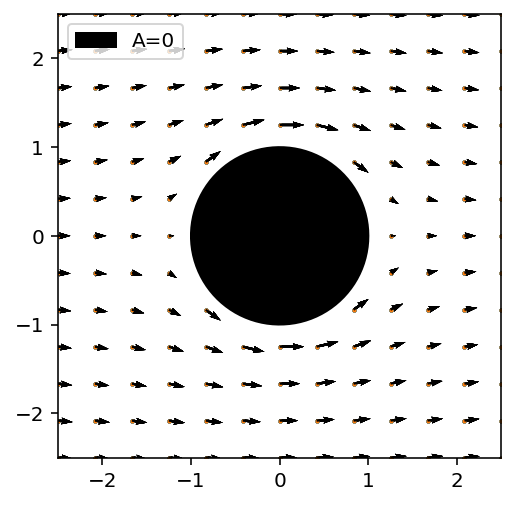
\includegraphics[width = 0.45\textwidth]{papers/joukowski/images/05_stroemungslinien/Magnus_Speed_A000.png}
\end{figure}

	\begin{figure}
	\centering
	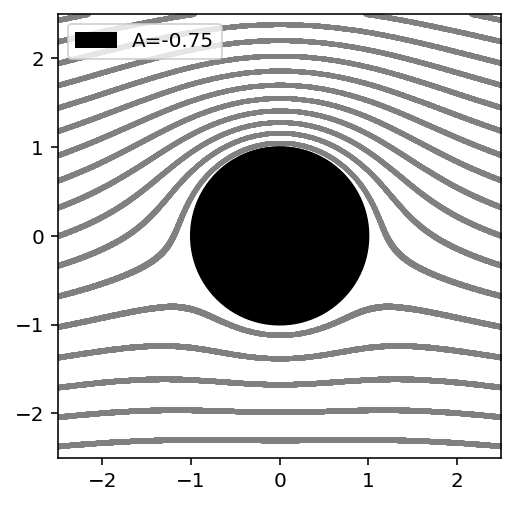
\includegraphics[width=0.45\textwidth]{papers/joukowski/images/05_stroemungslinien/Magnus_Strom_A075_g.png}
	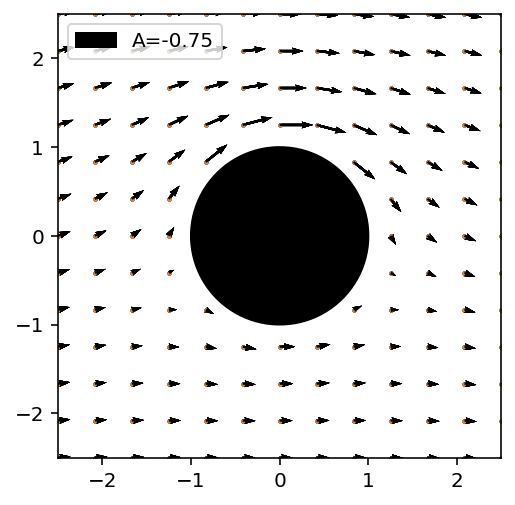
\includegraphics[width = 0.45\textwidth]{papers/joukowski/images/05_stroemungslinien/Magnus_Speed_A075.png}
\end{figure}

	\begin{figure}
	\centering
	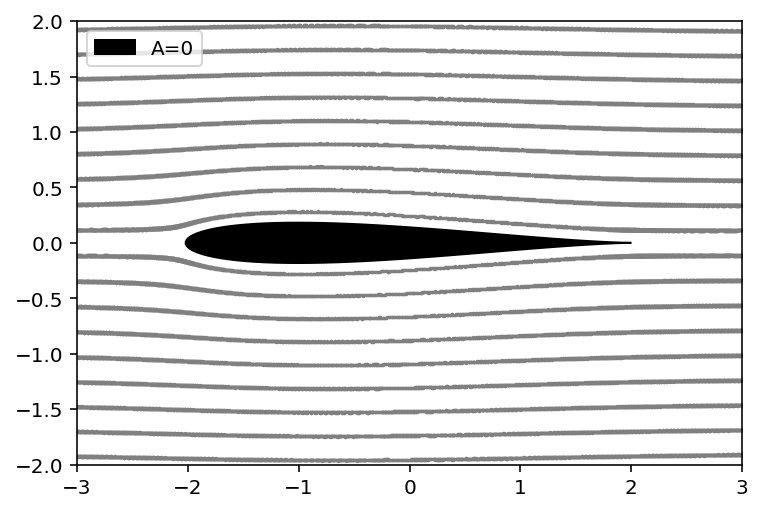
\includegraphics[width=0.6\textwidth]{papers/joukowski/images/05_stroemungslinien/fluegel_strom_A000_V04_g.png}
%	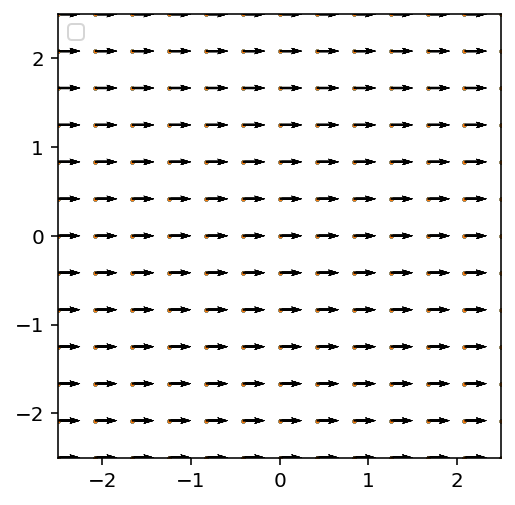
\includegraphics[width = 0.45\textwidth]{papers/joukowski/images/05_stroemungslinien/speed.png}
	\caption{
		\label{joukowski:Stroemungslinien:fig_fluegel1}
	}
\end{figure}

	\begin{figure}
	\centering
	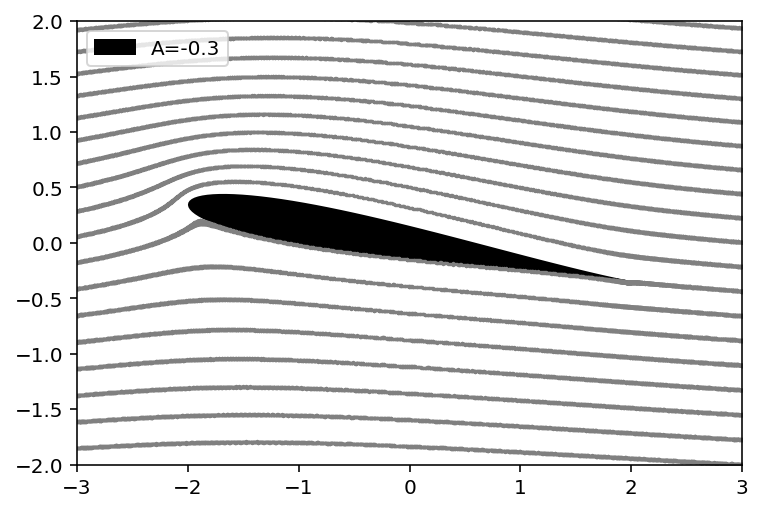
\includegraphics[width=0.6\textwidth]{papers/joukowski/images/05_stroemungslinien/fluegel_strom_A030_Rot_V02_g.png}
%	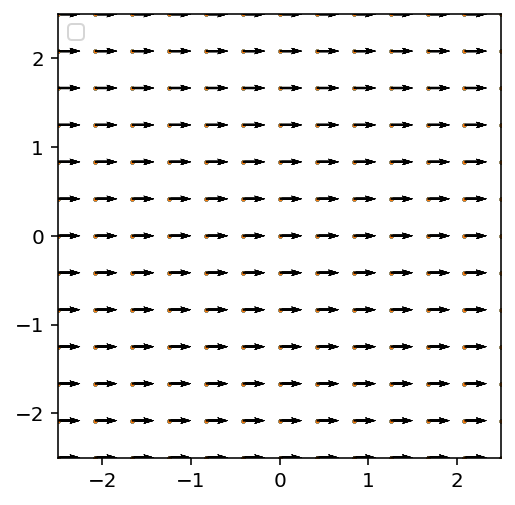
\includegraphics[width = 0.45\textwidth]{papers/joukowski/images/05_stroemungslinien/speed.png}
	\caption{
		\label{joukowski:Stroemungslinien:fig_fluegel2}
	}
\end{figure}

	
\label{joukowski:sec:stroemungslinien}
	\subsection{Allgemeine Definition}
		Um ein Verständnis dafür aufzubauen, wie die Luft um ein Flügelprofil strömt, muss zunächst ein grundlegendes Verständnis einer Strömung sowie ihres Geschwindigkeitsvektorfeldes vorhanden sein. In diesem Kapitel liegt der Fokus darauf, das Verständnis von Strömungen zu festigen und die mathematische Beschreibung einer Strömung in der komplexen Ebene aufzuzeigen.
		
		Beginnen wir mit einer Strömung, welche ungehindert von links nach rechts strömen kann. Es wird sofort deutlich, dass die Strömungslinien gleichmässig verteilt sind und das Geschwindigkeitsvektorfeld homogen und konstant ist. Somit ist die Geschwindigkeit an jedem Punkt des Raumes gleich. Die Abbildung ~\eqref{joukowski:Stroemungslinien:fig_Allgemein}, welche dieser Situation entspricht, kann mit dem Ausdruck $f(z) = z$ und $v(z) = 1$ beschrieben werden. Die Punkte in der Z-Ebene, welche in die Funktion $f(z)$ eingesetzt einen konstanten Imaginärteil ergeben, nennen wir eine Strömungslinie. Dieses Konzept ist für alle weiteren Anwendungen anwendbar.
		
		In einem weiteren Beispiel fügen wir einen Zylinder als Hindernis ein. Die Funktion, welche einen Kreis auf eine horizontale Linie abbildet, lautet $f(z) = z+\frac{1}{z}$. Für das Geschwindigkeitsvektorfeld wird lediglich die Ableitung benötigt. Die Funktion $v(z)$ lautet somit $v(z) = 1 - 1/z^2$. Die Strömungslinien dieser Funktion werden in Abbildung ~\eqref{joukowski:Stroemungslinien:fig_Zylinder} dargestellt.
	 
	\subsection{Magnus Effekt}
	\subsection{Tragflügel}
	\subsection{Vom Modell zum Koeffizienten}
		Mithilfe des Modells kann gezeigt werden, das der Parameter A, von der Form 	$f_s(z) = \frac{k}{2}\cdot(z+\frac{1}{z})-i\cdot A\cdot \log(z)$ \\, Numerisch ermittelt werden kann. Des weiteren kennen wir die vereinfachte Formel für den Auftrieb ~\eqref{joukowski:komplexe-analysis:auftriebskraft-berechnet}. Wir sind uns unsicher wie wir von A auf den Parameter a1 schliessen können.
	